\chapter{Модель активации теплоносителя первого контура}

\section{Миграция радионуклидов на \ac{aes}}
\label{sec_nuclides_migration}

Как и любое масштабное производство, \ac{aes} выбрасывает в атмосферу и окружающую среду вредные вещества, среди 
которых есть и радиоактивные. При нормальных условиях эксплуатации эти выбросы незначительны, так как современные 
атомные электростанции содержат множество систем очистки сбросов от радионуклидов, однако при нарушении работы 
какой-либо из систем \ac{aes} становится серьезным источником выбросов радионуклидов в атмосферу. 

Хотя принцип работы различных типов ядерных реакторов одинаков, их технологические схемы и устройства различны. В 
данном разделе рассмотрим образование радионуклидов с дальнейшим переходом в теплоноситель первого контура на примере 
реактора типа \ac{vver}.

Основные пути распространения радиоактивных нуклидов на \ac{aes} представлены на рисунке \ref{fig_nuclides_spread}.

\begin{figure}[ht]
\centering
	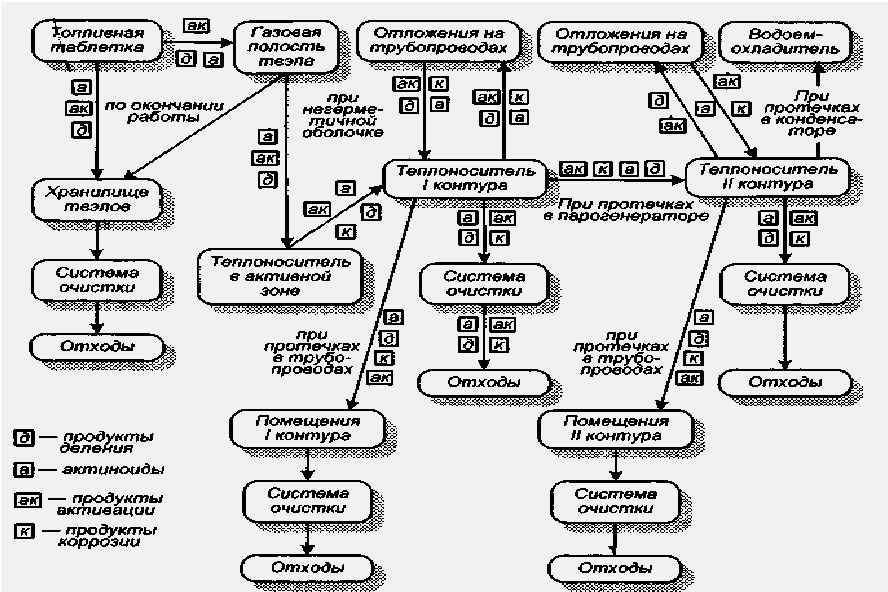
\includegraphics[width=16cm]{nuclides_spread}
	\captionsetup{justification=centering}
    \caption{Основные пути распространения радионуклидов на \ac{aes}.}
    \label{fig_nuclides_spread}
\end{figure}

Топливную таблетку в \ac{tvel}ах рассматривают как первый барьер распространения радиоактивных нуклидов в пределах 
активной зоны ядерного реактора. В результате реакции деления и захвата нейтронов в топливной таблетке накапливаются 
радионуклиды, изменяя состав, физико-химические и механические свойства топливной композиции. При температуре ниже 
1000 \degree C диоксид урана, который наиболее часто используется в качестве топлива в реакторах типа \ac{vver}, 
удерживает все радионуклиды, образующиеся в процессе работы реактора. При росте температуры ситуация существенно 
меняется, так как продукты захвата и деления становятся более подвижными \cite{leskin_vver}.

Между топливной таблеткой и оболочкой \ac{tvel}а присутствует небольшой зазор и газовая полость, предназначенные для 
накопления продуктов деления и активации, которым удалось покинуть пределы топливной таблетки.

Вторым барьером распространения радионуклидов является оболочка \ac{tvel}ов. В случае герметичной оболочки \ac{tvel}ов 
выход радионуклидов за пределы оболочки достаточно мал. В реальности, из за высоких тепловых и радиационных нагрузок и 
процессов коррозионно-усталостного типа оболочки теряют свою герметичность. Согласно \cite{kolpakov_tvel}, при 
эксплуатации ядерного реактора пределом безопасной эксплуатации по количеству и величине дефектов составляет 1 \% 
\ac{tvel}ов с дефектами типа газовой неплотности.

В случае разгерметизации топливной оболочки радионуклиды диффундируют через микротрещины в теплоноситель, находящийся 
в активной зоне реактора, который в дальнейшем переходит в первый контур реакторной установки. Более того, 
дополнительным источником радиоактивности в теплоносителе первого контура является его активация нейтронами. 

При эксплуатации \ac{aes} в нормальном режиме работы обеспечивается локализация радиоактивных продуктов деления, 
продуктов активации в реакторной установке и основных системах очистки от радиоактивных нуклидов. Парогенератор и 
трубопроводы первого и второго контуров не позволяют значительной части радионуклидов покинуть основные барьеры. Однако
при наличии микротрещин или протечек в парогенераторе радиоактивность первого контура может перейти в теплоноситель 
второго контура реакторной установки. В то же время, при протечках в трубопроводах первого или второго контура 
радионуклиды попадают в технические помещения, а далее загрязненный воздух через вентиляционные системы выбрасывается 
в атмосферу. Газообразные выбросы с \ac{aes} перед попаданием в атмосферу проходят сложную систему очистки, которая в 
свою очередь необходима для снижения активности выбросов, а далее попадают в окружающую среду через высокую трубу.

Помимо газообразных радиоактивных отходов при работе реактора выделяются жидкие и твердые отходы (рисунок 
\ref{fig_nuclides_spread2}). Твердыми радиоактивными отходами являются конструкционные материалы из активной зоны и 
первого контура, фильтры очистки установок, загрязненные инструменты, приборы и т.д. Твердые радиоактивные отходы после 
эксплуатации отправляются на захоронение. Жидкие радиоактивные отходы также образуются в результате эксплуатации 
\ac{aes}, в дальнейшем их очищают, разбавляют, фильтруют или концентрируют и хранят в специальных емкостях в жидком 
виде, однако при протечках в парогенераторе и конденсаторе радиоактивные отходы, мигрировавшие во второй контур 
реакторной установки, могут попасть в водоем-охладитель \cite{bekman_nuclear}. 

\begin{figure}[ht]
	\centering
	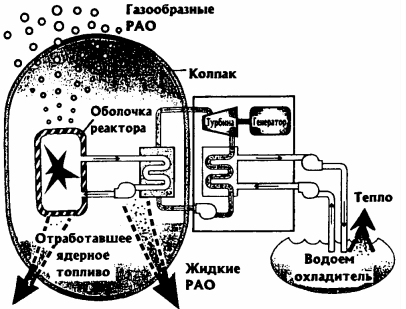
\includegraphics[width=10cm]{nuclides_spread2}
	\captionsetup{justification=centering}
    \caption{Схема образования газообразных, жидких и твердых отходов от \ac{aes} \cite{bekman_nuclear}.}
    \label{fig_nuclides_spread2}
\end{figure}

\section{Образование газообразных радионуклидов \ac{aes}}
\label{sec_gas_nuclides}

Рассмотрим наиболее важные радионуклиды, которые образуются в процессе работы реакторной установки и потенциально 
могут попасть в атмосферу путем газообразных выбросов \ac{aes}. В качестве топлива рассматривается изотоп $^{235}U$.

\subsection{Инертные радиоактивные газы}

Важную роль в формировании радиационной обстановке в районе выбросов \ac{aes} являются инертные радиоактивные газы 
(\ac{irg}). \ac{irg} попадают в теплоноситель при разгерметизации оболочек \ac{tvel}ов путем диффузии. Более десятка 
нуклидов инертных радиоактивных газов (криптона и ксенона) образуется в процессе деления нейтронами ядерного топлива 
\cite{bekman_nuclear}, а так же при распаде других продуктов реакции деления. Часть радионуклидов имеют либо малый 
период полураспада (меньше минуты), либо вносят ничтожно малый вклад в суммарную активность, из-за чего их можно не 
учитывать в расчетах. В реакторах типа \ac{vver} инертные радиоактивные газы могут поступать в атмосферу путем утечки 
воды из первого контура реакторной установки или при утечке воды из второго контура реакторной установки при протечках в 
парогенераторе.

Среди радиоактивных изотопов ксенона, образующихся в процессе работы реактора, выделяют $^{133}Xe$, $^{135}Xe$, $^{137}Xe$, 
$^{138}Xe$ \cite{gusev_bio}. Образование всех перечисленных изотопов в работающем реакторе происходит в результате деления 
ядерного топлива. Существует 2 основных канала образования изотопов ксенона. Ксенон образуется в результате распада 
изотопов йода ($^{133}I$, $^{135}I$, $^{137}I$, $^{138}I$), которые, в свою очередь, также образуются в результате распада 
изотопов теллура ($^{133}Te$, $^{135}Te$, $^{137}Te$, $^{138}Te$), являющихся продуктами реакции деления топлива. Также 
есть вероятность образования изотопов ксенона непосредственно в результате реакции деления ядерного топлива.

Цепочки распадов и образования изотопов ксенона, а так же информация о периодах полураспада и относительных выходах 
продуктов реакции деления, представлены на рисунках \ref{fig_xe_133_decay} --- \ref{fig_xe_138_decay}.

\begin{figure}[ht!]
    \centering
    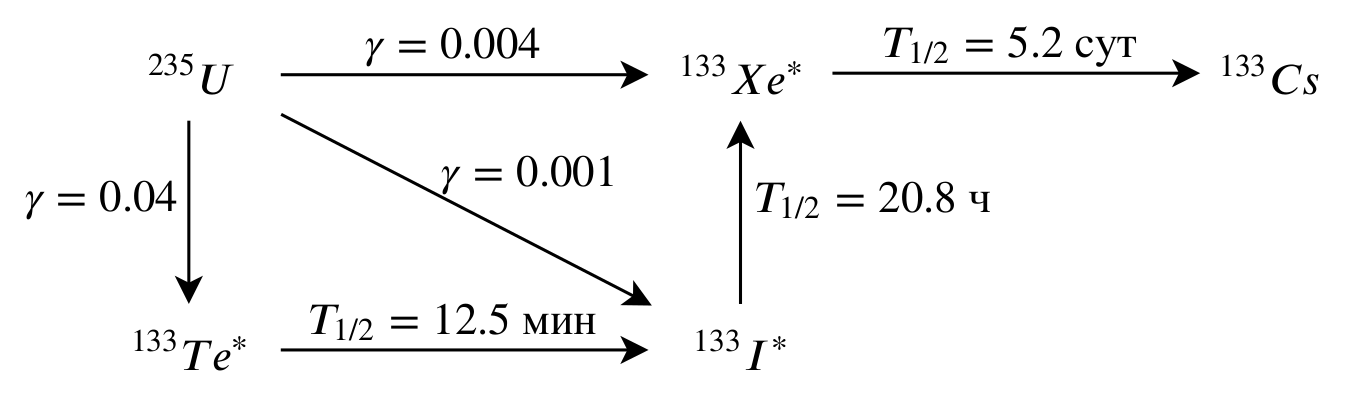
\includegraphics[width=13cm]{decay_xe_133}
    \captionsetup{justification=centering}
    \caption{Цепочка образования изотопа $^{133}Xe$ \cite{periodic_table}.}
    \label{fig_xe_133_decay}
\end{figure}

\begin{figure}[ht!]
    \centering
    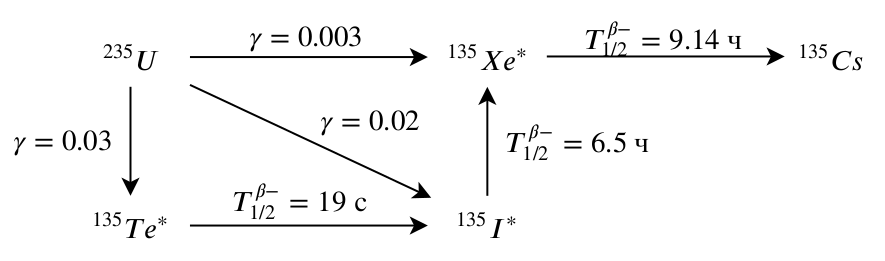
\includegraphics[width=13cm]{decay_xe_135}
    \captionsetup{justification=centering}
    \caption{Цепочка образования изотопа $^{135}Xe$ \cite{periodic_table}.}
    \label{fig_xe_135_decay}
\end{figure}

\begin{figure}[ht!]
    \centering
    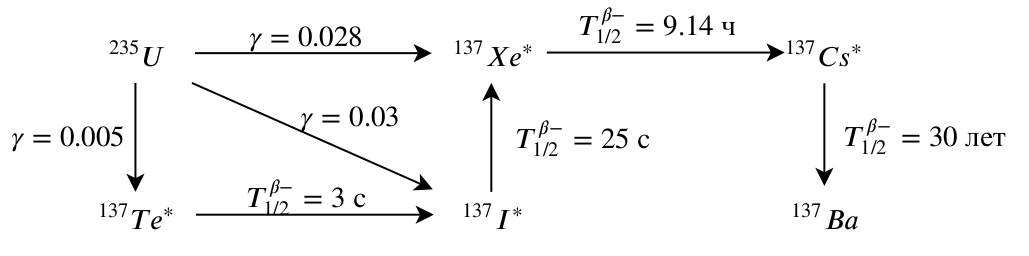
\includegraphics[width=13cm]{decay_xe_137}
    \captionsetup{justification=centering}
    \caption{Цепочка образования изотопа $^{137}Xe$ \cite{periodic_table}.}
    \label{fig_xe_137_decay}
\end{figure}

\begin{figure}[ht!]
    \centering
    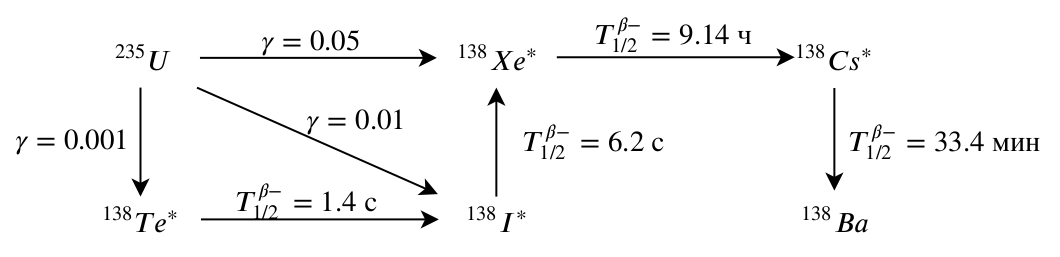
\includegraphics[width=13cm]{decay_xe_138}
    \captionsetup{justification=centering}
    \caption{Цепочка образования изотопа $^{138}Xe$ \cite{periodic_table}.}
    \label{fig_xe_138_decay}
\end{figure}

Важными изотопами криптона, образующимися во время работы реактора, являются изотопы $^{85}Kr$, $^{87}Kr$, $^{88}Kr$ 
\cite{gusev_bio}. Их образование также происходит в результате реакции деления ядерного топлива по двум основным каналам: 
во-первых при распаде изотопов $^{85}Br$, $^{87}Br$, $^{88}Br$, которые, в свою очередь, образуются в результате распада 
изотопов $^{85}Se$, $^{87}Se$, $^{88}Se$, являющихся продуктами реакции деления топлива.

Цепочки распадов и образования изотопов криптона, а так же информация о периодах полураспада и относительных выходах 
продуктов реакции деления, представлены на рисунках \ref{fig_kr_85_decay} --- \ref{fig_kr_87_decay}. 

\begin{figure}[ht!]
    \centering
    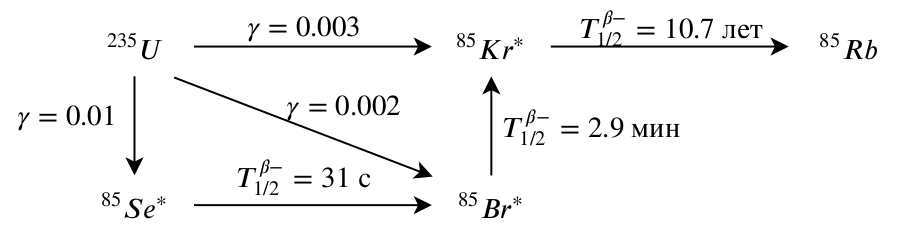
\includegraphics[width=13cm]{decay_Kr_85}
    \captionsetup{justification=centering}
    \caption{Цепочка образования изотопа $^{85}Kr$ \cite{periodic_table}.}
    \label{fig_kr_85_decay}
\end{figure}

\begin{figure}[ht!]
    \centering
    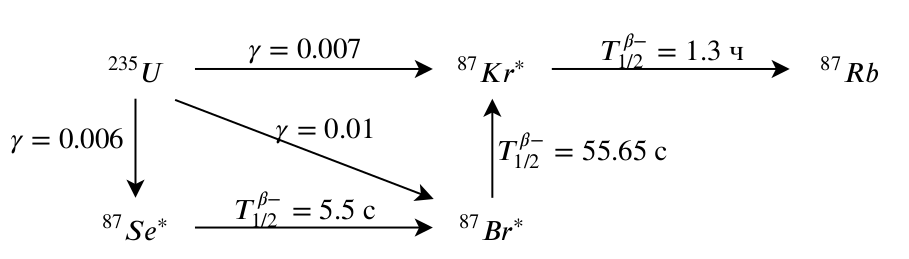
\includegraphics[width=13cm]{decay_Kr_87}
    \captionsetup{justification=centering}
    \caption{Цепочка образования изотопа $^{87}Kr$ \cite{periodic_table}.}
    \label{fig_kr_87_decay}
\end{figure}

\begin{figure}[ht!]
    \centering
    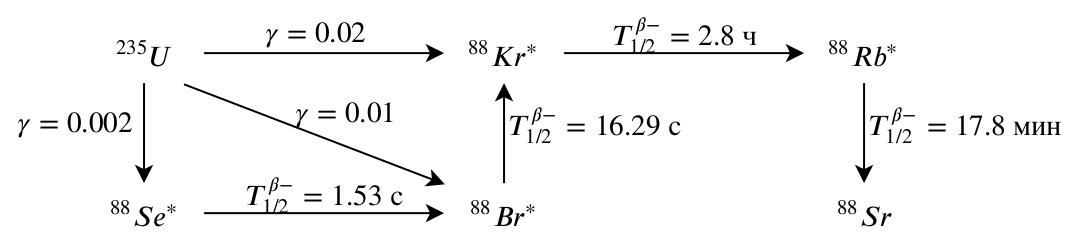
\includegraphics[width=13cm]{decay_Kr_88}
    \captionsetup{justification=centering}
    \caption{Цепочка образования изотопа $^{88}Kr$ \cite{periodic_table}.}
    \label{fig_kr_88_decay}
\end{figure}

Стоит отметить, что радионуклиды, период полураспада которых намного меньше кампании реактора ($^{137}\text{Xe}, 
^{87}\text{Kr}$), в ходе работы реактора быстро достигают состояния насыщения и их количество не меняется со временем. В 
то же время долгоживущие радионуклиды, период полураспада которых близок или превышает кампанию реактора 
($^{85}\text{Kr}$), накапливаются в топливе практически линейно со временем \cite{naumov_security}.

\subsection{Изотопы йода}

Не менее важными газообразными радионуклидами, попадающими в атмосферу, являются изотопы йода. Наиболее важными изотопами 
йода, образующимися во время работы реактора, являются изотопы $^{131}I$, $^{132}I$, $^{133}I$, $^{134}I$, $^{135}I$ 
\cite{gusev_bio}. Все перечисленные изотопы образуются либо в качестве продуктов деления ядерного топлива, либо как 
продукты распада изотопов $^{131}Te$, $^{132}Te$, $^{133}Te$, $^{134}Te$, $^{135}Te$. Пути попадания радиоактивных 
изотопов йода в атмосферу аналогичны инертным радиоактивным газам. Цепочки образования изотопов $^{133}I$ и $^{135}I$ 
представлены на рисунках \ref{fig_xe_133_decay} и \ref{fig_xe_135_decay}, а изотопов $^{131}I$, $^{132}I$, $^{134}I$ 
на рисунках \ref{fig_I_131_decay} - \ref{fig_I_134_decay} соответственно.

\begin{figure}[ht!]
    \centering
    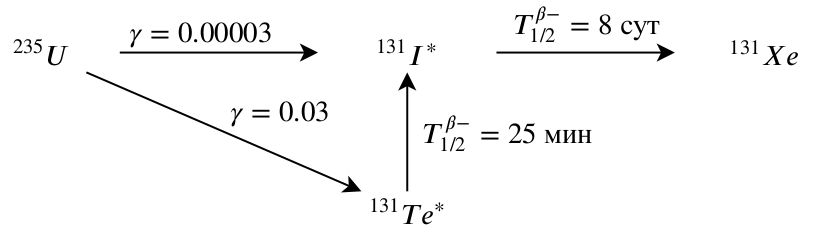
\includegraphics[width=13cm]{decay_I_131}
    \captionsetup{justification=centering}
    \caption{Цепочка образования изотопа $^{131}I$ \cite{periodic_table}.}
    \label{fig_I_131_decay}
\end{figure}

\begin{figure}[ht!]
    \centering
    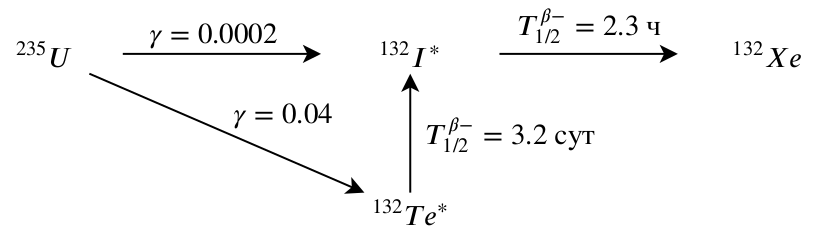
\includegraphics[width=13cm]{decay_I_132}
    \captionsetup{justification=centering}
    \caption{Цепочка образования изотопа $^{132}I$ \cite{periodic_table}.}
    \label{fig_I_132_decay}
\end{figure}

\begin{figure}[ht!]
    \centering
    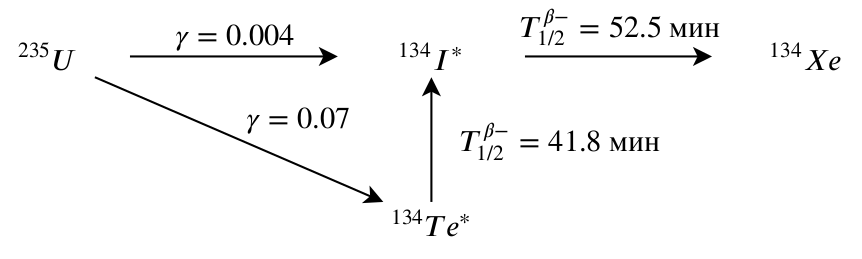
\includegraphics[width=13cm]{decay_I_134}
    \captionsetup{justification=centering}
    \caption{Цепочка образования изотопа $^{134}I$ \cite{periodic_table}.}
    \label{fig_I_134_decay}
\end{figure}

Из-за небольшого периода полураспада, в реакторе для вышеперечисленных радионуклидов достаточно быстро устанавливается 
равновесное состояние. Исключение составляет изотоп $^{129}\text{I}$ ($\text{T}_{1/2} = 1.57 \times  10^7$ лет), однако 
согласно \cite{bekman_nuclear} долгоживущий йод не обнаруживают в атмосфере и окружающей среде вокруг \ac{aes} и его 
выбросы во много раз меньше выбросов других радионуклидов йода.

\subsection{Аэрозоли}

Некоторые продукты деления ядер топлива, продукты распада \ac{irg} и радионуклиды с наведенной активностью образуют 
аэрозоли, которые попадают во внешнюю среду с воздушными потоками. Наиболее важными радионуклидами, входящими в 
состав аэрозольных выбросов с реактора типа \ac{vver}, являются $^{88}\text{Rb}$, $^{134}\text{Cs}$, $^{137}\text{Cs}$, 
$^{138}\text{Cs}$, $^{60}\text{Co}$. 

Изотоп $^{88}\text{Rb}$ образуется в реакторе в результате распада изотопа $^{88}\text{Kr}$, а также в результате 
реакции деления ядерного топлива с относительным выходом $\gamma=0.0004$ \cite{gusev_bio}. Цепочка образования 
$^{88}\text{Rb}$ представлена на рисунке \ref{fig_kr_88_decay}.

Изотоп $^{134}\text{Cs}$ образуется в реакторе в результате реакции деления ядерного топлива, а также в результате 
захвата нейтрона стабильным изотопом $^{133}\text{Cs}$, который образуется в реакторе в результате распада изотопа 
$^{133}\text{Xe}$ как показано на рисунке \ref{fig_xe_133_decay}. Цепочки образования изотопа $^{134}\text{Cs}$, а также 
информация о периодах полураспада и относительных выходах продуктов реакции деления, представлены на рисунке 
\ref{fig_Cs_134_decay} \cite{gusev_bio}.

\begin{figure}[ht!]
    \centering
    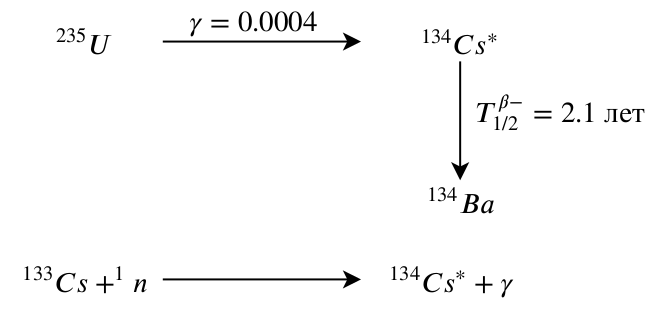
\includegraphics[width=10cm]{decay_Cs_134}
    \captionsetup{justification=centering}
    \caption{Цепочки образования изотопа $^{134}Cs$ \cite{periodic_table}.}
    \label{fig_Cs_134_decay}
\end{figure}

Изотопы $^{137}\text{Cs}$ и $^{138}\text{Cs}$ образуются в реакторе в результате реакции деления ядерного топлива с 
относительными долями выхода $\gamma=0.0008$ и $\gamma=0.001$ соответственно. Также рассматриваемые изотопы цезия 
образуются в результате распада изотопов $^{137}\text{Xe}$ и $^{137}\text{Xe}$, как было показано на рисунках 
\ref{fig_xe_137_decay} - \ref{fig_xe_138_decay} \cite{gusev_bio}.

Изотоп $^{60}\text{Co}$ образуется в реакторе в результате активации продукта коррозии конструкционных материалов 
$^{59}\text{Co}$. Накопление изотопа $^{59}\text{Co}$ в реакторе происходит в результате длительной и многократной 
циркуляции теплоносителя в первом контуре реакторной установки. Цепочка образования изотопа $^{60}\text{Co}$ 
представлена на рисунке \ref{fig_Co_60_decay} \cite{gusev_bio}.

\begin{figure}[ht!]
    \centering
    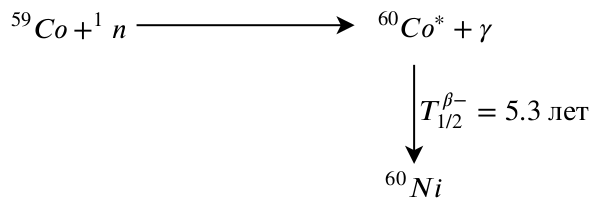
\includegraphics[width=10cm]{decay_Co_60}
    \captionsetup{justification=centering}
    \caption{Цепочка образования изотопа $^{60}Co$ \cite{periodic_table}.}
    \label{fig_Co_60_decay}
\end{figure}

\subsection{Активационные газы}

В процессе работы реактора при облучении стабильных изотопов нейтронами образуются активационные газы. Важнейшими 
активационными газами являются изотопы $^{16}\text{N}$ и $^{41}\text{Ar}$ \cite{gusev_bio}. 

Изотоп $^{16}\text{N}$ образуется в реакторе при облучении нейтронами стабильного изотопа $^{16}\text{O}$, который 
содержится в реакторе типа \ac{vver} в оксидном топливе, а также в теплоносителе \cite{gusev_bio}. Цепочка образования 
изотопа $^{16}\text{N}$ представлена на рисунке \ref{fig_N_16_decay}.

\begin{figure}[ht!]
    \centering
    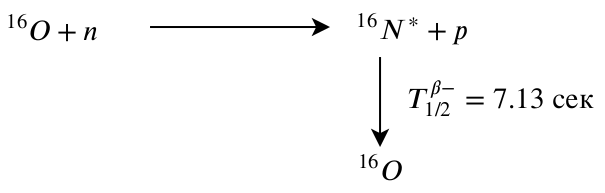
\includegraphics[width=10cm]{decay_N_16}
    \captionsetup{justification=centering}
    \caption{Цепочка образования изотопа $^{16}N$ \cite{periodic_table}.}
    \label{fig_N_16_decay}
\end{figure}

Изотоп $^{41}\text{Ar}$ образуется при облучения нейтронами изотопа $^{40}\text{Ar}$, растворенного в теплоносителе 
вместе с воздухом \cite{gusev_bio}. Цепочка образования изотопа $^{41}\text{Ar}$ представлена на рисунке 
\ref{fig_Ar_41_decay}.

\begin{figure}[ht!]
    \centering
    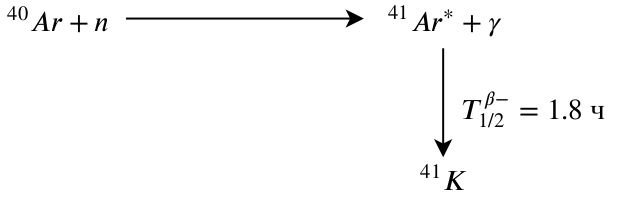
\includegraphics[width=10cm]{decay_Ar_41}
    \captionsetup{justification=centering}
    \caption{Цепочка образования изотопа $^{41}Ar$ \cite{periodic_table}.}
    \label{fig_Ar_41_decay}
\end{figure}

\subsection{Углерод}

Радиоактивный углерод $^{14}\text{C}$ образуется в реакторе по трём основным каналам: активация нейтронами естественных 
карбидных солей в теплоносителе первого контура, содержащих $^{13}\text{C}$; активация азота $^{14}\text{N}$; активация 
кислорода, содержащегося в оксидном топливе и в теплоносителе первого контура \cite{bekman_nuclear}. Цепочки образования 
изотопа $^{14}\text{C}$ представлены на рисунке \ref{fig_C_14_decay}.

\begin{figure}[ht!]
    \centering
    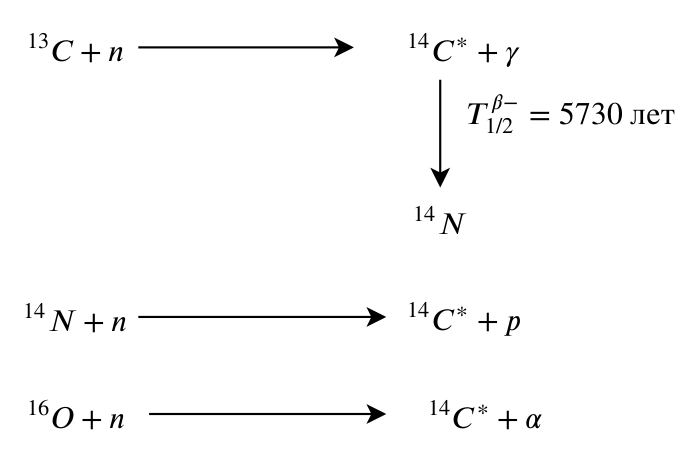
\includegraphics[width=10cm]{dacay_C_14}
    \captionsetup{justification=centering}
    \caption{Цепочки образования изотопа $^{14}C$ \cite{periodic_table}.}
    \label{fig_C_14_decay}
\end{figure}

\subsection{Тритий}

Газообразный тритий $^{3}\text{H}$ образуется в реакторе по двум основным каналам: при тройном делении ядер топлива и в 
ходе активации дейтерия, содержащегося в теплоносителе в качестве примеси \cite{bekman_nuclear}. Цепочки образования 
изотопа $^{3}\text{H}$ представлены на рисунке \ref{fig_H_3_decay}.

\begin{figure}[ht!]
    \centering
    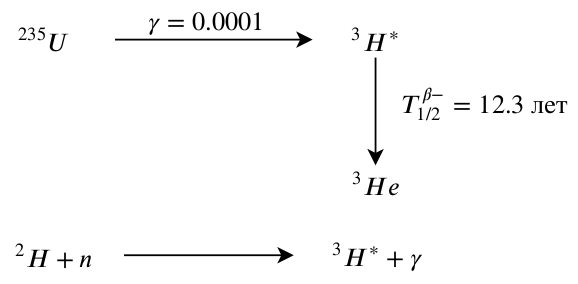
\includegraphics[width=10cm]{decay_H_3}
    \captionsetup{justification=centering}
    \caption{Цепочки образования изотопа $^{3}H$ \cite{periodic_table}.}
    \label{fig_H_3_decay}
\end{figure}

\section{Активация теплоносителя радионуклидами, выходящими из под оболочки \ac{tvel}ов}
\label{sec_tvel_nuclides}

Как было сказано в разделе \ref{sec_gas_nuclides}, в случае разгерметизации оболочек \ac{tvel}ов в теплоноситель 
первого контура могут попасть следующие радионуклиды, образующиеся в результате реакции деления ядер топлива: изотопы 
йода ($^{131}\text{I}$, $^{132}\text{I}$, $^{133}\text{I}$, $^{134}\text{I}$, $^{135}\text{I}$), изотопы, входящие в 
состав аэрозолей ($^{134}\text{Cs}$, $^{137}\text{Cs}$, $^{138}\text{Cs}$, $^{88}\text{Rb}$), инертные радиоактивные 
газы ($^{133}\text{Xe}$, $^{135}\text{Xe}$, $^{137}\text{Xe}$, $^{138}\text{Xe}$, $^{85}\text{Kr}$, $^{87}\text{Kr}$, 
$^{88}\text{Kr}$), а так же тритий ($^{3}\text{H}$).

Изменение концентрации i-ого нуклида, который образуется под оболочкой твэла в результате деления, определяется формулой 
\ref{eq_tvel_conc}.

\begin{equation}
    \label{eq_tvel_conc}
    \frac{\partial c_{i}}{\partial t} = -\lambda_{i}c_{i} + \gamma_{i}\Sigma_{f}\phi - S_{i}
\end{equation}

где:
\begin{description}
    \item $\text{c}_i$ --- концентрация i-го нуклида под оболочкой \ac{tvel}а;
    \item $\lambda_{i}$ ---  постоянная распада i-ого нуклида;
    \item $\gamma_{i}$ --- вероятность выхода i-ого нуклида при реакции деления;
    \item $\Sigma_{f}$ --- макроскопическое сечение деления ядер топлива;
    \item $\phi$ --- поток нейтронов;
    \item $\text{S}_{i}$ --- скорость выхода i-ого нуклида из-под оболочки \ac{tvel}а.
\end{description}

В левой части уравнения \ref{eq_tvel_conc} - скорость изменения концентрации i-ого нуклида под оболочкой \ac{tvel}а, 
которая представлена в виде суммы трех слагаемых: скорости распада нуклида, скорости образования нуклида в результате 
деления ядер топлива и скорости увода нуклида через микротрещина разгерметизированных оболочек \ac{tvel}ов в 
теплоноситель первого контура.

Уравнение \ref{eq_coolant_balance} описывает баланс между концентрацией i-ого нуклида в теплоносителе первого контура 
без учета его очистки и выходом i-ого нуклида из-под оболочки \ac{tvel}ов:

\begin{equation}
    \label{eq_coolant_balance}
    S_{i}^{0} = \lambda_{i}\widetilde{c}_{i}^{0}\frac{V_{coolant}}{V_{core}}
\end{equation}

где:
\begin{description}
    \item $\widetilde{c}_{i}^{0}$ --- равновесная концентрация i-ого нуклида в теплоносителе первого контура;
    \item $S_{i}^{0}$ --- равновесный выход i-ого нуклида из-под оболочки \ac{tvel}ов, при котором в 
        теплоносителе первого контура будет установлена концентрация $\widetilde{c}_{i}^{0}$ i-ого нуклида;
    \item $V_{coolant}$ --- объем теплоносителя первого контура;
    \item $V_{core}$ --- объем активной зоны.
\end{description}

Выход радионуклидов через оболочку зависит от множества параметров. Для упрощения ограничимся зависимостью выхода от 
концентрации примеси в \ac{tvel}ах, давления в теплоносителе первого контура и числа поврежден­ных \ac{tvel}ов. 
Зависимость выхода i-ого радионуклида из-под оболочки \ac{tvel}ов представлена в формуле \ref{eq_tvel_quite}:

\begin{equation}
    \label{eq_tvel_quite}
    S_{i} = S_{i}^{0}F_{i}(c_{i}, P, N_{failedRods})
\end{equation}

где:
\begin{description}
    \item $P$ --- давление в теплоносителе первого контура;
    \item $N_{failedRods}$ --- количество поврежденных \ac{tvel}ов;
    \item $F_{i}$ --- функция, учитывающая отклонение значение выхода i-ого нуклида из-под оболочки \ac{tvel}а от 
        равновесного при изменении любого из её параметров.
\end{description}

Отметим, что функция $F_{i}(c_{i}, P, N_{failedRods})$ в модели определяется таким образом, что $S_{i}$ соответствует 
равновесному выходу i-ого радионуклида при номинальном режиме работы реакторной установки. Иначе говоря, при отсутствии 
поврежденных \ac{tvel}ов, а так же при давлении в первом контуре, соответствующем номинальному давлению и достижении 
равновесного значения концентрации i-ого радионуклида под оболочкой \ac{tvel}а функция $F_{i}(c_{i}, P, N_{failedRods})$ 
равна 1.

Изменение концентрации радионуклидов в теплоносителе первого контура определяется формулой \ref{eq_coolant_conc}:

\begin{equation}
    \label{eq_coolant_conc}
    \frac{\partial \widetilde{c}_{i}}{\partial t} = -\lambda_{i}\widetilde{c}_{i} + S_{i}
\end{equation}

Учитывая выражения \ref{eq_coolant_balance} и \ref{eq_tvel_quite} преобразуем уравнение \ref{eq_coolant_conc} к виду 
\ref{eq_coolant_conc_2}:

\begin{equation}
    \label{eq_coolant_conc_2}
    \frac{\partial \widetilde{c}_{i}}{\partial t} = -\lambda_{i}\widetilde{c}_{i} + \lambda_{i}\widetilde{c}_{i}^{0}F_{i}
\end{equation}

Представим функцию $F_{i}$ в виде произведения четырёх сомножителей (формула \ref{eq_F_i}):

\begin{equation}
    \label{eq_F_i}
    F_{i} = Z_{i}K_{i}Q_{i}M_{i}
\end{equation}

где:
\begin{description}
    \item $Z_{i}$ --- функция, определяющая зависимость выхода радионуклидов из-под оболочки \ac{tvel}ов от количества 
        поврежденных \ac{tvel}ов;
    \item $K_{i}$ --- функция, определяющая зависимость выхода радионуклидов из-под оболочки \ac{tvel}ов от давления в 
        активной зоне ядерного реактора;
    \item $Q_{i}$ --- функция, определяющая зависимость выхода радионуклидов из-под оболочки \ac{tvel}ов от концентрации 
        i-ого радионуклида под оболочкой \ac{tvel}ов;
    \item $M_{j}$ --- функция, учитывающая изменение плотности теплоносителя в $j$-ом расчетном ноде от средней 
        плотности при номинальной мощности реактора.
\end{description}

Функция $Z_{i}$ определяется как линейная функция от числа поврежденных \ac{tvel}ов (формула \ref{eq_Z_i}):

\begin{equation}
    \label{eq_Z_i}
    Z_{i} = 1 + z_{i}N_{failedRods}
\end{equation}

где:
\begin{description}
    \item $z_{i}$ --- коэффициент, определяющий увеличение концентрации  i-ого радионуклида при повреждении одного 
        \ac{tvel}а.
\end{description}

Функция $K_{i}$ определяется как дробно-линейная функция \ref{eq_K_i}:

\begin{equation}
    \label{eq_K_i}
    K_{i} = (\frac{P_{0}}{P})^{\alpha_{i}}
\end{equation}

где:
\begin{description}
    \item $P$ --- текущее давление в первом контуре реакторной установки;
    \item $P_{0}$ --- давление в первом контуре реакторной установки в номинальном режиме работы;
    \item $\alpha_{i}$ --- степенной показатель, принятый в модели равным $1,5$.
\end{description}

Функция $Q_{i}$ определяется как дробно-линейная функция \ref{eq_Q_i}:

\begin{equation}
    \label{eq_Q_i}
    Q_{i} = \frac{c_{i}}{c_{i}^{0}}
\end{equation}

Функция $M_{j}$ зависит от плотности теплоносителя в j-ом расчетном ноде и определяется как отношение суммарной массы 
теплоносителя в активной зоне к массе теплоносителя в расчетном ноде (формула \ref{eq_M_j}). В текущей модели активная 
зона реактора разбивается на 27 эквивалентных каналов в разрезе и 20 высотных слоев, то есть индекс j проходит от 1 до 
$27 \times 20 = 540$.

\begin{equation}
    \label{eq_M_j}
    M_{j} = \frac{\sum_{j=1}^{540} V_{j}\overline{\rho}}{V_{j}\rho_{j}}
\end{equation}

где:
\begin{description}
    \item $V_{j}$ --- объем j-ого расчетного нода;
    \item $\overline{\rho}$ --- средняя плотность теплоносителя в активной зоне при номинальной мощности реактора;
    \item $\rho_{j}$ --- плотность теплоносителя в j-ом расчетном ноде.
\end{description}

В итоге, подставляя формулы \ref{eq_Z_i} -- \ref{eq_M_j} в выражение \ref{eq_F_i}, а получившееся выражение в 
\ref{eq_coolant_conc_2}, получим уравнение \ref{eq_coolant_conc_3}:

\begin{equation}
    \label{eq_coolant_conc_3}
    \frac{\partial \widetilde{c}_{i}}{\partial t} = -\lambda_{i}\widetilde{c}_{i} + \lambda_{i}\widetilde{c}_{i}^{0}
        (1 + z_{i}N_{failedRods})\frac{c_{i}}{c_{i}^{0}}\frac{\sum_{j=1}^{540} V_{j}\overline{\rho}}{V_{j}\rho_{j}}
        (\frac{P_{0}}{P})^{\alpha_{i}}
\end{equation}

Определим равновесную концентрацию i-ого радионуклида под оболочкой \ac{tvel}ов. В случае герметичной оболочки 
\ac{tvel}а выход радионуклидов из-под оболочки пренебрежимо мал, из за этого слагаемым в правой части уравнения 
\ref{eq_tvel_conc}, отвечающим за увод радионуклидов из-под оболочки, можно пренебречь. Тогда выражение 
\ref{eq_tvel_conc} принимает вид \ref{eq_tvel_conc_no_fail_rods}: 

\begin{equation}
    \label{eq_tvel_conc_no_fail_rods}
    \frac{\partial c_{i}}{\partial t} = -\lambda_{i}c_{i} + \gamma_{i}\Sigma_{f}\phi
\end{equation}

В результате временной дискретизации уравнения \ref{eq_tvel_conc_no_fail_rods} получим формулу \ref{eq_tvel_conc_time_discr}:

\begin{equation}
    \label{eq_tvel_conc_time_discr}
    c_{i}(t) = \frac{c_{i}(t - \Delta t) + \gamma_{i} \Sigma_{f} \phi \Delta t}{1 + \lambda_{i} \Delta t}
\end{equation}

В текущей модели используется внесистемная единица измерения плотности потока нейтронов $\text{Вт/см}^{2}$, из-за чего 
плотность потока нейтронов необходимо дополнительно умножить на коэффициент $k$, который представлен в формуле 
\ref{eq_k}:

\begin{equation}
    \label{eq_k}
    k = \frac{\nu_{f}}{E_{f}}
\end{equation}

где:
\begin{description}
    \item $\nu_{f}$ --- выход нейтронов на одно деление ядер топлива;
    \item $E_{f}$ --- энергия, выделяемая в результате одного деления ядер топлива (Дж).
\end{description}

Учитывая этот коэффициент, выражение \ref{eq_tvel_conc_time_discr} принимает вид \ref{eq_tvel_conc_time_discr_2}:

\begin{equation}
    \label{eq_tvel_conc_time_discr_2}
    c_{i}(t) = \frac{c_{i}(t - \Delta t) + \gamma_{i} \Sigma_{f} k \phi \Delta t}{1 + \lambda_{i} \Delta t}
\end{equation}

Приравняв в выражении \ref{eq_tvel_conc_no_fail_rods} частную производную концентрации радионуклидов по времени к 
нуклю получим равновесную концентрацию i-ого нуклида под оболочкой \ac{tvel}а (формула \ref{eq_tvel_equilibrium_conc}):

\begin{equation}
    \label{eq_tvel_equilibrium_conc}
    c_{i}^{0} = \frac{\gamma_{i} \Sigma_{f} k \phi}{\lambda_{i}} 
\end{equation}

Активность радионуклида определяется как количество распадов нуклида в единицу времени \cite{gusev_def}. Активность 
i-ого радионуклида в теплоносителе связана с концентрацией радионуклида через постоянную распада (формула 
\ref{eq_activ}):

\begin{equation}
    \label{eq_activ}
    \widetilde{A_{i}} = \lambda_{i} \widetilde{c}_{i}
\end{equation}

Учитывая формулу \ref{eq_activ} преобразуем выражение \ref{eq_coolant_conc_3}. Результат представлен в конечной формуле 
\ref{eq_coolant_conc_4}:

\begin{equation}
    \label{eq_coolant_conc_4}
    \frac{\partial \widetilde{c}_{i}}{\partial t} = -\widetilde{A_{i}} + \widetilde{A_{i}^{0}}
        (1 + z_{i}N_{failedRods})\frac{c_{i}}{c_{i}^{0}}\frac{\sum_{j=1}^{540} V_{j}\overline{\rho}}{V_{j}\rho_{j}}
        (\frac{P_{0}}{P})^{\alpha_{i}}
\end{equation}

где:
\begin{description}
    \item $\widetilde{A_{i}}$ --- активность i-ой примеси в теплоносителе 1-ого контура;
    \item $\widetilde{A_{i}^{0}}$ --- равновесная активность i-ой примеси в теплоносителе первого контура.
\end{description}

Значения равновесных активностей и другие характеристики радионуклидов, образующихся в топливе, использующиеся в 
текущей модели, приведены в приложении Б.

\section{Образование радионуклидов в теплоносителе под действием облучения}

\subsection{Расчетная модель}

Помимо выхода радионуклидов из-под оболочки \ac{tvel}ов, описанного в разделе \ref{sec_tvel_nuclides}, активация 
теплоносителя первого контура в реакторной установке происходит из-за облучения естественных примесей теплоносителя и 
продуктов коррозии конструкционных материалов. 

В текущей модели активации естественных примесей теплоносителя и продуктов коррозии учитывается образование следующих 
радионуклидов: $^{16}\text{N}$, $^{41}\text{Ar}$, $^{3}\text{H}$, $^{14}\text{C}$.

При расчете концентрации естественных примесей в теплоносителе в модели применяется допущение, что эта концентрация 
остается постоянной со временем. Такое допущение обуславливается тем, что естественные примеси являются стабильными, а 
под действием облучения лишь небольшая часть примесей претерпевает ядерные превращения. Расчет концентраций естественных 
примесей в теплоносителе первого контура производится по формуле \ref{eq_natural_mix}:

\begin{equation}
    \label{eq_natural_mix}
    \widetilde{c_{i}^{n}} = p_{i}^{n} \frac{N_{a}}{M_{H_{2}O}}
\end{equation}

где:
\begin{description}
    \item $\widetilde{c_{i}^{n}}$ --- массовая концентрация i-ого нуклида естественной примеси (ядер/кг теплоносителя);
    \item $p_{i}^{n}$ --- доля i-ого нуклида естественной примеси в теплоносителе первого контура;
    \item $N_{a}$ --- число Авогадро;
    \item $M_{H_{2}O}$ --- молярная масса воды (кг/моль).
\end{description}

Скорость изменения i-ого радионуклида в теплоносителе рассчитывается по формуле \ref{eq_natural_conc}:

\begin{equation}
    \label{eq_natural_conc}
    \frac{\partial \widetilde{c}_{i}}{\partial t} = -\lambda_{i}\widetilde{c}_{i} + \sigma_{i}^{n,j} \widetilde{c_{i}^{n}}
        \phi 
\end{equation}

где:
\begin{description}
    \item $\widetilde{c_{i}}$ --- концентрация i-ого радионуклида, образующегося в результате облучения естественных 
        примесей, входящих в состав теплоносителя первого контура;
    \item $\sigma_{i}^{n,j}$ --- микроскопическое сечение реакции типа j на ядре i-ого нуклида, входящего в состав 
        естественной примеси.
\end{description}

Для большей точности вычислений энергетическая область разбивается на 2 группы: быстрая и тепловая. Для расчета потоков 
нейтронов для быстрой и тепловой групп используется асимптотическая жесткость спектра нейтронов 
(формула \ref{eq_flux_group}):

\begin{equation}
    \label{eq_flux_group}
    \phi^{(1)} = \phi \frac{1}{1 + \zeta}, \phi^{(2)} = \phi \frac{\zeta}{1 + \zeta}
\end{equation}

где:
\begin{description}
    \item $\phi^{(1)}$ --- поток нейтронов быстрой группы;
    \item $\phi^{(2)}$ --- поток нейтронов тепловой группы;
    \item $\zeta$ --- асимптотическая жесткость спектра.
\end{description}

Учитывая формулы \ref{eq_k}, \ref{eq_activ}, \ref{eq_flux_group}, перепишем уравнение \ref{eq_natural_conc} в виде 
\ref{eq_natural_conc_2}:

\begin{equation}
    \label{eq_natural_conc_2}
    \frac{\partial \widetilde{c}_{i}}{\partial t} = -\widetilde{A}_{i} + \sigma_{i}^{(1), n,j} \widetilde{c_{i}^{n}}
        k \phi \frac{1}{1 + \zeta} + \sigma_{i}^{(2), n,j} \widetilde{c_{i}^{n}} k \phi \frac{\zeta}{1 + \zeta}
\end{equation}

где:
\begin{description}
    \item $\widetilde{A}_{i}$ --- активность i-ого радионуклида в теплоносителе первого контура;
    \item $\sigma_{i}^{(1), n,j}$ --- микроскопическое сечение для нейтронов быстрой энергетической группы реакции типа 
        j на ядре i-ого изотопа, входящего в состав естественных примесей;
    \item $\sigma_{i}^{(2), n,j}$ --- микроскопическое сечение для нейтронов тепловой энергетической группы реакции типа 
        j на ядре i-ого изотопа, входящего в состав естественных примесей; 
\end{description}

\subsection{Расчет концентрации радионуклида N-16}

Нуклид $^{16}\text{N}$ образуется в результате реакции (n, p) на ядре $^{16}\text{O}$. Эта реакция является 
пороговой и идет только на быстрых нейтронах с порогом около 10,2 МэВ. Изотоп $^{16}\text{O}$ является стабильным и 
входит в состав молекулы воды, следовательно доля данного изотопа в теплоносителе первого контура равна единице. 
Зависимость сечения реакции (n, p) на ядре $^{16}\text{O}$ от энергии представлена в приложении В. Двухгрупповые 
сечения реакции (n, p) на ядре $^{16}\text{O}$ были получены при помощи программы UNK \cite{unk}.

Учитывая формулу \ref{eq_natural_conc_2} и пороговый характер реакции (n, p), скорость изменения концентрации 
$^{16}\text{N}$ представлена формулой \ref{eq_n16}:

\begin{equation}
    \label{eq_n16}
    \frac{\partial \widetilde{c}_{N16}}{\partial t} = -\widetilde{A}_{N16} + \sigma_{O16}^{(1), (n, p)} \widetilde{c_{O16}}
        k \phi \frac{1}{1 + \zeta}
\end{equation}

где:
\begin{description}
    \item $\sigma_{O16}^{(1), (n, p)}$ --- сечение реакции (n, p) на ядре $^{16}\text{O}$ для быстрой группы нейтронов 
        ($1,029 \times 10^{-29}$ барн \cite{unk}).
\end{description}

\subsection{Расчет концентрации радионуклида Ar-41}

В качестве естественной примеси в теплоносителе содержится нуклид $^{40}\text{Ar}$, доля которого на кубометре пресной 
воды составляет $7 \times 10^{-6} \%$. При (n, $\gamma$) реакции на ядре изотопа $^{40}\text{Ar}$ образуется радионуклид 
$^{41}\text{Ar}$. Зависимость сечения реакции (n, p) на ядре $^{40}\text{Ar}$ от энергии представлена в 
приложении В. Двухгрупповые сечения реакции (n, $\gamma$) на ядре $^{40}\text{Ar}$ были получены при помощи программы 
UNK: 
$\sigma_{Ar40}^{(1), (n, \gamma)} = 5,22 \times 10^{-27}$ барн, 
$\sigma_{Ar40}^{(2), (n, \gamma)} = 2,93 \times 10^{-25}$ барн.

Расчет концентрации $^{41}\text{Ar}$ в теплоносителе первого контура производится по формуле \ref{eq_natural_conc_2}.

\subsection{Расчет концентрации радионуклида H-3}

Как было рассмотрено в разделе \ref{sec_gas_nuclides}, газообразный тритий в реакторе образуется по двум основным 
каналам: при тройном делении ядер топлива и в результате активации дейтерия в ходе реакции (n, $\gamma$). 

Расчет концентрации $^{3}\text{H}$ в теплоносителе первого контура, образующегося в результате реакции (n, $\gamma$) на 
ядре $^{2}\text{H}$ производится по формуле \ref{eq_natural_conc_2}. Доля дейтерия в теплоносителе первого контура 
составляет $2,3 \times 10^{-2} \%$ на кубический метр. Двухгрупповые сечения реакции (n, $\gamma$) на ядре 
$^{2}\text{H}$ были посчитаны при помощи программы UNK: 
$\sigma_{H2}^{(1), (n, \gamma)} = 2,467 \times 10^{-28}$ барн, 
$\sigma_{H2}^{(2), (n, \gamma)} = 3,549 \times 10^{-30}$ барн. 
Зависимость сечения реакции (n, $\gamma$) на ядре $^{2}\text{H}$ от энергии представлена в приложении В.

\subsection{Расчет концентрации радионуклида C-14}

Согласно разделу \ref{sec_gas_nuclides}, радиоактивный углерод образуется в реакторе по трем основным каналам. 
Рассмотрим каждый из них.

Во-первых, изотоп $^{14}\text{C}$ образуется в результате реакции (n, $\gamma$) на стабильном изотопе $^{13}\text{С}$, 
который содержится в виде естественных карбидных солей в теплоносителе первого контура. Концентрация карбидных солей на 
дистиллированную воду составляет $5 \times 10^{-3} \text{кг/м}^{3}$ \cite{gost_water}. Доля изотопа $^{13}\text{C}$ в 
смеси стабильных изотопов $^{13}\text{C}$ и $^{12}\text{C}$ составляет $0,0107$ \cite{audi_carbid_sald}, следовательно 
концентрация изотопа $^{13}\text{C}$ в теплоносителе первого контура составляет $5 \times 10^{-5} \text{кг/м}^{3}$, а 
доля данного изотопа составляет $p_{C13} = \frac{\rho_{C13}}{\rho_{H_{2}O}} = 5,01 \times 10^{-6} \%$. Двухгрупповые 
сечения реакции (n, $\gamma$) на ядре $^{13}\text{C}$ были посчитаны при помощи программы UNK:
$\sigma_{C13}^{(1), (n, \gamma)} = 4,472 \times 10^{-28}$ барн, 
$\sigma_{C13}^{(2), (n, \gamma)} = 1,497 \times 10^{-27}$ барн.
Зависимость сечения реакции (n, $\gamma$) на ядре $^{13}\text{C}$ от энергии представлена в приложении В. 

Во-вторых, изотоп $^{14}\text{C}$ образуется в результате реакции (n, p) на ядре $^{14}\text{N}$. Суммарная концентрация 
аммониевых солей и нитратов на дистиллированную воду составляет $2 \times 10^{-5} \text{кг/м}^{3}$ \cite{gost_water}, 
следовательно доля $^{14}\text{N}$ в теплоносителе первого контура составляет 
$p_{N14} = \frac{\rho_{N14}}{\rho_{H_{2}O}} = 2,004 \times 10^{-6} \%$. Двухгрупповые сечения реакции (n, p) на ядре 
$^{14}\text{N}$ были посчитаны при помощи программы UNK:
$\sigma_{N14}^{(1), (n, p)} = 1,974 \times 10^{-26}$ барн, 
$\sigma_{N14}^{(2), (n, p)} = 2,337 \times 10^{-25}$ барн.
Зависимость сечения реакции (n, p) на ядре $^{14}\text{N}$ от энергии представлена в приложении В.

В третьих, изотоп $^{14}\text{C}$ образуется в результате реакции (n, $\alpha$) на ядре $^{17}\text{O}$. Доля изотопа 
$^{17}\text{O}$ в смеси стабильных изотопов кислорода составляет $0,037 \%$ \cite{hoefs_oxygen_isotopes}.

Для расчета микроскопического сечения реакции (n, $\alpha$) на изотопе $^{17}\text{O}$ в тепловой области энергий 
используется закон $\frac{1}{V}$ по формуле \ref{eq_1_div_V}:

\begin{equation}
    \label{eq_1_div_V}
    \sigma_{O17}^{(2), (n, \alpha)} = \sigma_{O17}^{0, (n, \alpha)} \frac{V_{th}^0}{V_{th}} = 
        \sigma_{O17}^{0, (n, \alpha)} \frac{1}{V_{th}} \sqrt{\frac{2 E_{th}^{0} k}{m_{n}}}
\end{equation}

где:
\begin{description}
    \item ${V_{th}}$ - текущая скорость тепловых нейтронов;
    \item ${V_{th}^{0}}$ - скорость тепловых нейтронов в тепловой точке ($2200$ м/с \cite{kruchkov_tpn});
    \item $E_{th}^{0}$ - энергия тепловых нейтронов в тепловой точке ($0,0253$ эВ \cite{kruchkov_tpn});
    \item $\sigma_{O17}^{0, (n, \alpha)}$ - сечение реакции (n, $\alpha$) при энергии тепловой точки ($4,986 \times 
        10^{-25}$ барн \cite{janis});
    \item $m_{n}$ - масса нейтрона ($1,675 \times 10^{-27}$ кг \cite{kruchkov_tpn});
    \item $k$ - коэффициент для перевод эВ в Дж ($1,60218 \times 10^{-19}$).
\end{description}

Для расчета микроскопического сечения реакции (n, $\alpha$) на изотопе $^{17}\text{O}$ в быстрой области энергий 
используется усреднение по спектру Ферми. Выбор спектра Ферми объясняется малым сечением поглощения нейтронов 
теплоносителем по сравнению с сечением рассеяния и малой концентрацией поглотителя $^{17}\text{O}$ в теплоносителе. 
Зависимость сечения реакции (n, $\alpha$) на ядре $^{17}\text{O}$ от энергии была взята из библиотеки TENDL-2017 
\cite{janis} и представлена в приложении В. Расчет производится по формуле \ref{eq_fermi}:

\begin{equation}
    \label{eq_fermi}
    \sigma_{O17}^{(1), (n, \alpha)} = \frac
        {\int_{0}^{E_{th}} \sigma_{O17}^{(n, \alpha)}(E) \phi^{F}(E) dE}
        {\int_{0}^{E_{th}} \phi^{F}(E) dE}, \phi^{F}(E) = \frac{1}{\zeta \rho_{H_2O} \sigma_{H_2O}^s E}
\end{equation}

где:
\begin{description}
    \item $E_{th}$ - граница тепловой области ($\sim 2$ эВ);
    \item $\phi^F(E)$ - спектр Ферми;
    \item $\zeta$ - среднелогарифмическая потеря энергии нейтрона при столкновении с ядрами воды ($0,948$ 
        \cite{savander_part1});
    \item $\rho_{H_2O}$ - плотность воды в реакторе ($720$ кг/м$^{3}$);
    \item $\sigma_{H_2O}^s$ - сечение рассеяния воды ($21 \times 10^{-24}$ барн \cite{janis}).
\end{description}

Результаты расчета микроскопических сечений реакции (n, $\alpha$) на изотопе $^{17}\text{O}$ представлены в приложении 
Г. Расчет концентрации $^{14}\text{C}$ в теплоносителе первого контура, образующегося в результате вышеперечисленных 
реакций, производится по формуле \ref{eq_natural_conc_2}.

\section{Заключение моделирования активации теплоносителя первого контура}

В данной главе была представлена модель образования радионуклидов в теплоносителе первого контура. Было представлено 2 
основных способа образования радионуклидов в теплоносителе: выход радионуклидов из-под оболочки \ac{tvel}ов и облучение 
естественных примесей теплоносителя первого контура с их дальнейшим превращением в радионуклиды.

При делении ядерного топлива образуются радиоактивные осколки, которые при разгерметизации оболочек \ac{tvel}ов могут 
перейти в теплоноситель первого контура. В текущей модели расчет концентрации радионуклидов, вышедших из-под оболочек 
\ac{tvel}ов в теплоноситель первого контура, производится по формуле \ref{eq_coolant_conc_4}. Основные характеристики 
радионуклидов, образующися в топливе, представлены в приложении Б.

В теплоносителе первого контура присутствуют естественные примеси, которые при облучении нейтронами могут перейти в 
радиоактивные нуклиды. В текущей модели расчет концентрации радионуклидов, образующихся в результате активации 
нейтронами естественных примесей теплоносителя первого контура, производится по формуле \ref{eq_natural_conc_2}. 
Параметры основных радионуклидов, образующихся в теплоносителе первого контура в результате активации нейтронами 
естественных примесей, представлены в приложении Г.


